\chapter{Common Peripheral Components}
\addcontentsline{lobb}{chapter}{\thechapter \hspace{0.2cm} Common Peripheral Components}
\label{chapter:Common Peripheral Components}
\graphicspath{ {./chapter10/Fig} }

The number and variety of devices available on the market
is truly astounding.  In this chapter you will be introduced
to some basic building blocks that you may want to use for
your projects in the future.

%% Input devices
\section{Pushbutton}
\index{push button|(}
    \label{page:pushbutton}
    \begin{buildingblock}{Push Button}
        \begin{tabular}{|l|p{3.5in}|} \hline
            Nomenclature:  & Pushbutton         \\ \hline
            Data Input:    & none         \\ \hline
            Data Output:   & none   \\ \hline
            Control:       & none           \\ \hline
            Status:        & none                                   \\ \hline
            Physical Input:& push button        \\ \hline
            Physical Output:& none        \\ \hline
            Others:        & 2 wires             \\ \hline
            Behavior:      & When the button is pressed a short circuit is created
            between the two terminals, otherwise there is an open circuit between
            the two terminals. \\ \hline
        \end{tabular}
    \end{buildingblock}

    A push button is perhaps the simplest input device that you will
    utilize in digital design.  Unfortunately you cannot just pop
    a pushbutton into a design by itself, it (like many other devices
    in this chapters) requires some support circuitry.
    Figure~\ref{fig:commonPeripheralComponentspushbutton} shows how to wire a normally open
    pushbutton so that it outputs a logic 0 when pressed, otherwise
    it outputs a logic 1.  The term normally open refers to the fact
    that the terminals of the button normally form an open circuit.
    When pressed the terminals form a short circuit.

    \begin{figure}[ht]
        \center{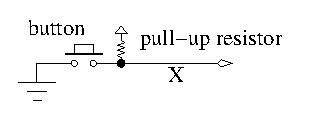
\includegraphics{pushbutton}}
        \caption{A push button with a pull-up resistor.}
        \label{fig:commonPeripheralComponentspushbutton}
    \end{figure}

    Usually, the button of a normally open push button will be colored
    red, the button of a normally closed button colored black.
    The figure shows that the right side of the button is connected to
    5 volts through a resistor; the value of the resistor is typically
    set to 4.7k$\Omega$.  The left side of the button is connected directly
    to ground.  The operation of this circuit is straight forward.  When
    the button is pressed the $X$ signal is tied directly to ground,
    hence $X=0$.  When the button is released (as shown in the figure)
    $X$ is connected to 5 volts through a resistor.  If we assume that
    $X$ is connected to a digital circuit with a high input impedance
    then $X=1$.

    \subsection{Switch Bouncing}
    No discussion of buttons (and switches) would be complete without
    mentioning signal bouncing.  In an ideal world when the button
    \index{switch bouncing|(}
        shown in Figure~\ref{fig:commonPeripheralComponentspushbutton} was pressed then output $X$
        would go solidly from 5 volts to ground.  Unfortunately, pushbuttons
        are mechanical devices with real mechanical limitations.  The contacts
        inside the pushbutton will literally bounce when contact is first
        made.  This bouncing will cause the voltage to oscillate as shown
        in Figure~\ref{fig:commonPeripheralComponentsbounce}.

        \begin{figure}[ht]
            \center{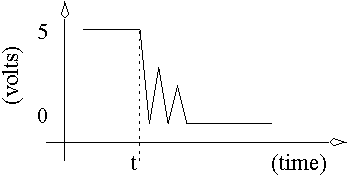
\includegraphics{bounce}}
            \caption{Signal bounce out of a pushbutton pressed at time $t$.}
            \label{fig:commonPeripheralComponentsbounce}
        \end{figure}

        Switch bouncing can be a major problem in digital circuits because
        the circuit sees the signal change several times and may take
        actions appropriate for each of these bounce values when the user
        only intended a single actions to take place.  There are a variety of
        methods used to get around this problem.  An electrical engineer
        might approach the problem by fitting a low pass filter to the
        output of the pushbutton circuit.  Since this is involves only a
        resistor and capacitor its a simple and attractive solution.  A
        computer engineer may elect for oversampling, whereby the output
        of the pushbutton is sampled several times and only when all the
        samples agree is the state of the pushbutton changes to the
        unanimous value.

        \subsection{Switch Interfacing}
        \label{page:push_dp}
        Frequently, you will be building digital circuits that interface with
        humans operating in the real world.  Unfortunately, humans and digital
        circuits involved operate at dramatically different frequencies.
        This time difference becomes important when a FSM must respond to
        human inputs.  For example, consider a circuit which counts the number
        of times that a button has been pressed using the circuit shown in
        Figure~\ref{fig:commonPeripheralComponentspush7button}.  Assume that the clock is running at
        8Mhz.

        \begin{figure}[ht]
            \center{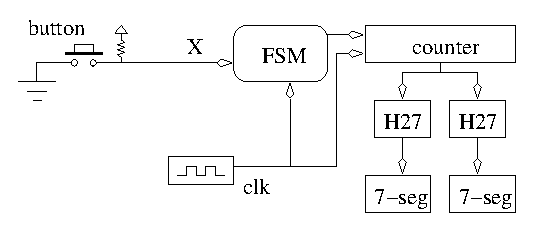
\includegraphics{pushbutton_dp}}
            \caption{A circuit to count the number of times a button is pushed.}
            \label{fig:commonPeripheralComponentspush7button}
        \end{figure}

        The output of the FSM drives the control inputs of an 8-bit counter.
        The output of the counter is sent to two hex to seven segment converts
        which send their output to a pair of 7-segment displays.
        The FSM needs to sample the button and on each push tell the counter
        to count up by 1.  At all other times the FSM should tell the counter
        to hold its count value.   Figure~\ref{fig:commonPeripheralComponentspushfsm}
        shows two possible state diagrams for the FSM.

        \begin{figure}[ht]
            \center{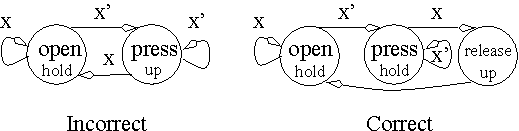
\includegraphics{pushfsm}}
            \caption{Two state diagrams for the pushbutton circuit.}
            \label{fig:commonPeripheralComponentspushfsm}
        \end{figure}

        Lets first examine the incorrect state diagram on the left.  It
        contains two states \textbf{ open, press}.  When the FSM is in state
        \textbf{ open} it outputs a 2-bit control signal to the counter
        telling it to hold.  When the FSM is in state \textbf{ press} the
        2-bit output tells the counter to count up.  This seems to be
        what the word statement asked for, except for one subtle point; digital
        circuits are much faster than humans.  This fact implies that
        a momentary button push by a human could easily last, say
        a million clock cycles for the FSM.  This implies that the FSM
        would stay in the \textbf{ press} state for a million clock cycles.
        Hence, the circuit would count up a million times.  We wanted
        our circuit to count up once for each button push.  Obviously,
        the state diagram on the left is not what we wanted.

        The solution to this problem is shown in the state diagram to
        the right.  The difference in this state diagram is the introduction
        of a third state, \textbf{ release}.  This state is entered when the
        push button is released and is exited on the next clock cycle.
        Thus, we spend only one clock cycle in the state in which the
        counter is told to increment.  The memory input equations and
        output equations are left as an exercise.
        Finally, we turn our attention to the value of the clock frequency.
        What should its value be set at?  There are two limits involved
        in the answer to this question.  The highest frequency is set by
        the propagation delays of the FSM and the counter.  Since we
        can reasonably assume that we have access to technologies on the
        order of 10's of megahertz we will use this as the upper limit
        to the frequency.  On the other hand, the lowest
        frequency must be greater than the fastest event your circuit
        is expected to see.  A safe bet would be to set the clock
        frequency equal to twice the frequency of the fastest event your
        circuit should be expected to see.   In this way the circuit
        will not miss any events of interest.

        \section{Three-State Buffer}
        \begin{buildingblock}{Three State Buffer}
            \label{buildingblock:threeStateBuffer}
            \index{three-state buffer|(}
                \begin{tabular}{|l|p{3.5in}|} \hline
                    Nomenclature:  & Three-state buffer    \\ \hline
                    Data Input:    & 1-bit X        \\ \hline
                    Data Output:   & 1-bit Y        \\ \hline
                    Control:       & 1-bit $c$              \\ \hline
                    Status:        & none            \\ \hline
                    Others:        & none            \\ \hline
                    Behavior:      & The output equals the input when
                    $C=1$ otherwise the output is
                    disconnected from input. \\ \hline
                \end{tabular}
                \label{page:tsb}
            \end{buildingblock}

            When several devices share a common signaling pathway, as with
            a data bus, it is important for every device to be capable of
            asserting data onto the bus, but only one device at a time
            actually asserts data.  This effect can only be accomplished if each
            device is capable of electrically disconnecting itself from the
            bus.  The three-state buffer shown in Figure~\ref{fig:comboBBtsb} does
            this under the control of the $c$ signal.

            \begin{figure}[ht]
                \begin{tabular}[b]{p{1.0in}p{0.5in}l}
                    \includegraphics[10mm,10mm][12mm,12mm]{tsb} & &

                    $
                    \begin{array}{c|c||c}
                        X & C & Y \\ \hline
                        x & 0 & Z \\ \hline
                        0 & 1 & 0 \\ \hline
                        1 & 1 & 1 \\
                    \end{array}$
                \end{tabular}
                \caption{The symbol and truth table for a three-state buffer.}
                \label{fig:comboBBtsb}
            \end{figure}

            Notice, when $C=1$, then $Y=X$; the output equals the
            input.  But, when $C=0$, the output equals $Z$.  $Z$ is
            a symbol commonly used in electrical engineering
            to refer to impedance (reciprocal of resistance).  The
            $Z$ means the output is not connected to anything.

            It is common to see $N$ three-state buffers organized together to
            produce an N-bit three-state buffer.  In such an arrangement,
            each bit of input is routed to its own three-state buffer,
            and the control input is routed to all of the three-state
            buffers.  Each three-state buffer contributes its one bit
            of output to the overall output from the N-bit three-state
            buffer.

            Directly connecting together outputs of two gates creates
            a situation where the two gates may produce different outputs
            resulting in a short circuit.  This connection will
            eventually lead to the failure of one or both of the gates.
            Clearly, a system should not be designed with such a flaw.
            However, cases arise when it makes sense to want to wire
            together the outputs of several gates.

            The bus \index{bus} in a computer is a collection
            of related signals that move information between any pair
            of devices on the bus.  Allowing a bus to be used by many
            different devices increases its utilization at the expense
            of increased complexity.  Look at the example bus in
            Figure~\ref{fig:comboBBbus} which connects a CPU, RAM, and Disk.
            Each of these devices may want data to be sent or
            received from any of the others.  The shaded box in each device
            (CPU, RAM, Disk) is called out on the right side of Figure~\ref{fig:comboBBbus}.
            The input register latches data from the bus and the output
            register holds the data to be asserted on the bus.  The
            three-state buffer can disconnect the output register from the bus
            allowing one of the other devices to assert data on the bus.
            It is important, and fairly obvious, that only one device at a
            time can assert data on the bus.

            \begin{figure}[ht]
                \center{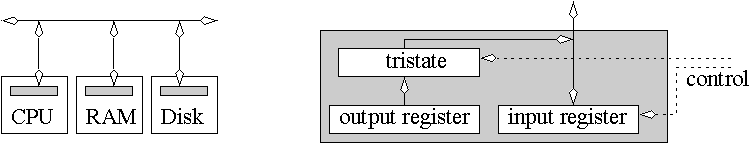
\includegraphics{bus}}
                \caption{Three devices on a bus.  The internal circuitry in
                each device to make it work.}
                \label{fig:comboBBbus}
            \end{figure}
        \index{three-state buffer|)}

        %\section{Switch Types}

        \section{Rotary Encoder}
        \index{rotary encoder|(}
            \label{page:rotary}
            \begin{buildingblock}{Rotary Encoder}
                \begin{tabular}{|l|p{3.5in}|} \hline
                    Nomenclature:  & Rotary Encoder                           \\ \hline
                    Data Input:    & none         \\ \hline
                    Data Output:   & 2-bit vector $A=a_1 a_0$   \\ \hline
                    Control:       & none           \\ \hline
                    Status:        & none                                   \\ \hline
                    Physical Input:& rotating knob        \\ \hline
                    Physical Output:& none        \\ \hline
                    Others:        & none                   \\ \hline
                    Behavior:      & When the encoders know is rotated clockwise (CW) the
                    vector $A$ produces an increasing gray code $00, 01, 11, 10, 00, ...$.
                    If the know is rotated CCW then the vector produces a decreasing gray
                    code $00,10,11,01,00, ...$. \\ \hline
                \end{tabular}
            \end{buildingblock}

            Rotary encoders are commonly used as the tuner knob on car radios.
            They have a distinctive feel, when turned they click into
            position.  Each of these clicks is called a detent.   A typical
            rotary encoder will have 32 detents per rotation.  Rotary encoders
            are capable of being turned endlessly,
            they have no rotation stops.  Typically, a rotary encoder will always have the
            same value, say 00, when it is in a detent.  When the knob is moved
            from one detent to the next the output of the encoder moves through
            a gray coded sequence.  The direction of the knob twist determine whether the
            output sequence is 00,01,11,10 or 00,10,11,01.   \index{gray code|(}
                Figure~\ref{fig:commonPeripheralComponentsencoder}A shows the physical appearance of a rotary
                encoder and the support circuitry necessary to operate one.

                \begin{figure}[ht]
                    \center{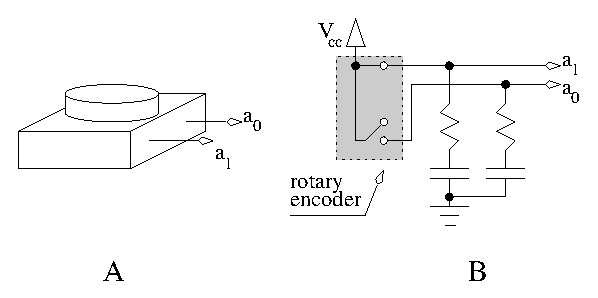
\includegraphics{encoder}}
                \caption{a) A physical rotary encoder.  B) The support circuitry for
            the encoder.}
            \label{fig:commonPeripheralComponentsencoder}
        \end{figure}

        Clearly, a rotary encoder is not able to produce logic levels out
        of thin air.   Figure~\ref{fig:commonPeripheralComponentsencoder}B shows the support
        circuitry consisting of resistors and capacitors connected to
        \VCC and GND.  In this schematic the rotary encoder is shown as the
        pair of switches in the shaded box.  The upper switch is closed
        forcing the voltage \VCC to be applied directly to $a_1$, hence its
        value is logic 1.  The lower switch is open, since no other voltage
        is being applied to $a_0$ the ground connection through the resistor
        "tugs" that line to logic 0.  The capacitors are installed to reduce
        switch bouncing.

        \section{Keyboard}
        \index{keyboard|(}
            \label{page:keyboad}
            \begin{buildingblock}{PS2 Keyboard}
                \begin{tabular}{|l|p{3.5in}|} \hline
                    Nomenclature:  & Keyboard                           \\ \hline
                    Data Input:    & none        \\ \hline
                    Data Output:   & 1-bit data and 1-bit clock   \\ \hline
                    Control:       & none           \\ \hline
                    Status:        & none                                   \\ \hline
                    Physical Input:& many keys        \\ \hline
                    Physical Output:& none        \\ \hline
                    Others:        & none                   \\ \hline
                    Behavior:      & When a key is pressed the keyboard sends a make code.
                    When a key is released the keyboard sends a break code followed by the
                    keys scan code. \\ \hline
                \end{tabular}
            \end{buildingblock}

            Computers are ubiquitous in today's society.  Despite being its primary
            data input mechanism, most people know very little about how a computers
            keyboard functions.  Foremost, a keyboard is a serial device, it transmits
            data 1 bit at a time.  Without some reference it would be impossible
            to differentiate one bit from the next.  Thus, in addition to its 1-bit
            data line a keyboard also outputs a clock signal.  Nominally, both the
            clock and data lines are held high (they are both open collector, the
            pull-up resistor being inside the keyboard).  The act of pressing and releasing
            a key causes three discrete packages of information to be transmitted from
            the keyboard as shown at the top of Figure~\ref{fig:commonPeripheralComponentskeyboard}.

            \begin{figure}[ht]
                \center{\scalebox{0.8}{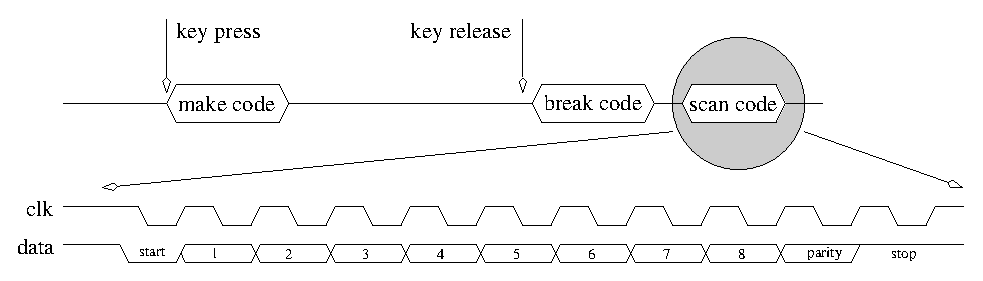
\includegraphics{keyboard}}}
                \caption{A timing diagram shown the relationship between the
                clock and data signals.}
                \label{fig:commonPeripheralComponentskeyboard}
            \end{figure}

            When you press a key on your keyboard the make code of the key is
            transmitted.  When the key is released a break code is sent immediately
            followed by the scan code of the key.  Each of these packets consists
            of 11-bits as shown in the lower half of Figure~\ref{fig:commonPeripheralComponentskeyboard}.
            The data from the keyboard is always valid on the falling edge of the
            clock signal; data is typically changed on or around the rising edge
            of the clock.  The 11-bit data packet always starts with a start-bit
            which always equals 0.  This bit is typically used to make sure that
            the clock signal didn't change because of noise.  Following the
            start bit are 8-bits of data, transmitted least significant bit first.
            Following the data bits is an odd parity bit, whose value is set by the
            keyboard so that the total number of 1's transmitted in the 8 data
            bits and the parity bit equals an odd number.  For example, if the
            8 data bits were 01100011, yielding a total of 4 1's then the parity
            bit would equal 1 so that the total number of 1's would be an odd
            number, in this case 5.  The parity bit can be used by the receiver
            to check if a single bit error occurred.  For example, in the above
            case if the parity bit was 0 then the receiver would know that a data
            or parity bit was corrupted.  It would be up to the receiver as
            to what action to take next.  Following the parity bit the final
            bit, the stop bit, is always a logic 1.

            The relationship between the keys on the keyboard and the 8-bit data
            value is not at all obvious.  Typically, characters are encoded using
            ASCII, but not so with keyboards.  They are endowed with their very
            own code which is refereed to as keyboard scan codes.
            Table~\ref{table:keyboard} is a short excerpt from the complete table.

            \begin{table}
                \begin{tabular}{l|l|l|l|l|l}
                    key & code    & key & code    & key & code \\ \hline \hline
                    a   & 0x1C    & b   & 0x32    & c   & 0x21    \\ \hline
                    d   & 0x23    & e   & 0x24    & f   & 0x2B    \\ \hline
                    g   & 0x34    & h   & 0x33    & i   & 0x43    \\ \hline
                    j   & 0x3B    & k   & 0x42    & l   & 0x4B    \\ \hline
                    m   & 0x3A    & n   & 0x31    & o   & 0x44    \\ \hline
                    p   & 0x4D    & q   & 0x15    & s   & 0x2D    \\ \hline
                    s   & 0x1B    & t   & 0x2C    & u   & 0x3C    \\ \hline
                    v   & 0x2A    & w   & 0x1D    & x   & 0x22    \\ \hline
                    y   & 0x35    & z   & 0x1A    & left shift & 0x12    \\
                \end{tabular}
                \caption{The scan codes for some keyboard keys.}
                \label{table:keyboard}
            \end{table}

            Its interesting to note that there are not codes for the capital
            letters.  The reason is that the shift key has its own scan
            code just like the letters.  When you type in a capital letter
            using a shift key (for example "Z") the following sequence of
            actions takes place.

            \begin{tabular} {l|l}
                action        &    keyboard response    \\ \hline \hline
                press shift    &    0x12            \\ \hline
                pressing z    &    0x1A            \\ \hline
                releasing shift    &    0xF0 0x12        \\ \hline
                releasing z    &    0xF0 0x1A        \\
            \end{tabular}

            Clearly, your computer must remember that the shift key was pressed
            in order to differentiate between the upper and lower case z.

            \section{Keypad}
            \index{keypad|(}
                \label{page:keypad}
                \begin{buildingblock}{Keypad}
                    \begin{tabular}{|l|p{3.5in}|} \hline
                        Nomenclature:  & 16-button keypad                           \\ \hline
                        Data Input:    & 4-bit row        \\ \hline
                        Data Output:   & 4-bit column   \\ \hline
                        Control:       & none           \\ \hline
                        Status:        & none                                   \\ \hline
                        Physical Input:& 16 buttons        \\ \hline
                        Physical Output:& none        \\ \hline
                        Others:        & none                   \\ \hline
                        Behavior:      & When a key is pressed a connection is made between
                        the corresponding row and column. \\ \hline
                    \end{tabular}
                \end{buildingblock}

                You probably used a keypad the last time that you dialed a phone.
                Keypads generally are laid out in a grid.
                For example, on the left side of Figure~\ref{fig:commonPeripheralComponentskeypad}
                is a keypad with 4 rows and 4 columns.  The internal organization
                of this keypad is shown to the right in this figure.  A keypad is
                nothing more than a set of switches, when a key is pressed a connection
                is made between the corresponding row and column.  For example, when
                the "6" key is pressed a connection is made between row 2 and column
                3.

                \begin{figure}[ht]
                    \center{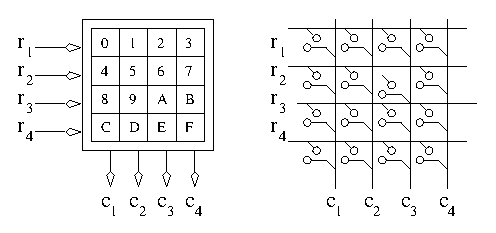
\includegraphics{keypad}}
                    \caption{A keypad and its internal circuit.}
                    \label{fig:commonPeripheralComponentskeypad}
                \end{figure}

                The operation of the keypad is straight forward.  Building a circuit
                which determines which key was pressed is more involved.   A common
                solution is to pull each column output to ground via a resistor.  Then
                one at a time, each row is driven to 5 volts using a decoder.  The
                columns are then monitored looking for a logic 1 denoting a key press
                between the currently active row and the column.  This process
                of activating a row and looking at the columns is called scanning.  The
                scanning process must be fast enough so that a quick key press can be
                detected.

                %% information output devices
                \section{Light Emitting Diodes}
                \index{led|(}
                    \label{page:led}
                    \begin{buildingblock}{Light Emitting Diode}
                        \begin{tabular}{|l|p{3.5in}|} \hline
                            Nomenclature: & LED \\ \hline
                            Data input:    & none     \\ \hline
                            Data output:   & none    \\ \hline
                            Control:       & none        \\ \hline
                            Status:        & none                                   \\ \hline
                            Physical Input:& none        \\ \hline
                            Physical Output:& light        \\ \hline
                            Others:        & An anode and a cathode                 \\ \hline
                            Behavior:      & When 2V is applied from the anode to the cathode the LED lights
                            up. \\ \hline
                        \end{tabular}
                    \end{buildingblock}

                    An LED is arguably the simplest output device.  Foremost a LED
                    is a diode (see Figure~\ref{fig:commonPeripheralComponentsled}A) which means that it is a
                    two terminal device which operates
                    in two modes.  When \textit{ forward biased} a higher voltage is applied
                    to the anode and a lower voltage applied to the cathode producing a
                    current flow through the diode.  In \textit{ reverse biased} mode the voltage
                    on the anode is not sufficiently higher than the voltage on the cathode,
                    hence no current flows.   The amount of current flowing through an LED
                    determines its brightness.
                    Typically LEDs require at least 1mA to produce a detectable
                    amount of light and at most 20mA at which point they are
                    distinctly brilliant.  The brightness of an LED is
                    quantified by how many millicandle (mcd) it produces.  A normal LED will
                    output around 2mcd at 10mA.  Another important parameter of an LED is the
                    amount of voltage dropped across it when it is forward biased, termed $V_f$.
                    For a normal LED, $V_f=2.0V$ whereas for a normal diode this value is
                    typically 0.7V.  A typical application of an LED is shown in
                    Figure~\ref{fig:commonPeripheralComponentsled}B.

                    \begin{figure}[ht]
                        \center{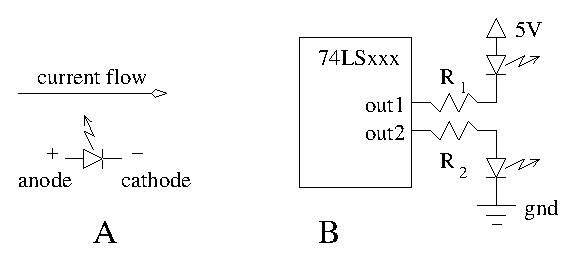
\includegraphics{led}}
                    \caption{A) The schematic representation of an LED.  B) Two LEDs wired
                to the output of a TTL device.}
                \label{fig:commonPeripheralComponentsled}
            \end{figure}

            The LED configurations driven by out1 and out2 are denoted active
            low and active high respectively.  An active low
            \index{active high|(}
                \index{active low|(}
                    output elicits its intended behavior when the output is at logic 0.
                    When out1 is at 5V there can is no voltage drop across the LED,
                    hence no light is emitted.  When out1 is at ground then there is
                    a 2V drop across the LED and a 3V drop across the resistor $R_1$.
                    Since current is
                    flowing into the chip when out1 is low we say that out1 is
                    \textit{ sinking} current when the output is low.  Now, out2 works in
                    completely the opposite manner.  When out2 is high there is a
                    2V drop across the LED and a 3V drop across $R_2$.  Since current
                    flows out of out2 we say that out2 \textit{ sources} current when its
                    output is high.  Since active high outputs are the most intuitive
                    way to configure an LED, most students wonder why anyone would
                    wire up an LE in an active low configuration.  The answer lies on
                    the third page of the data sheet; \IOL > \IOH.  This means
                    that a typical TTL output can sink more current than it can source.
                    Since the brightness of an LED is determine by the amount of current
                    run through an LED, LEDs are generally wired up to TTL outputs
                    in an active low configuration.

                    It is useful to think of the resistor in either configuration as
                    "absorbing" the left over voltage not used by the LED.  The resistors
                    other main function is set the current
                    flowing through the LED.  If $R_1 = 1k \Omega$ then the current
                    through the resistor must be $3V/1k \Omega = 3mA$.  Clearly, any
                    current which flows through the resistor must flow through the
                    LED, hence the LED will be dimly illuminated with 3mA of current.
                    Decreasing the resistance of a
                    resistor will allow more current to flow through the LED and hence
                    make the LED brighter.  However, the process of decreasing the
                    resistance value cannot be continued indefinitely.  Either the 20mA
                    current limit of the LED will be reached or the current rating of
                    the chips will be reached.

                    \subsection{Pulse Width Modulation}
                    Living in a digital domain, one can get in the habit of thinking about
                    the world in terms of 0/1, true/false and on/off.  However, there are
                    techniques that can be used to  give a digital output a more "analog"
                    feel.  Pulse width modulation (PWM) is one of these techniques whereby
                    the average power delivered to a device is altered by changing the
                    duty cycle of the driving voltage.  For example, in Figure~\ref{fig:commonPeripheralComponentspulse}
                    a LED is connected to a TTL device in an active high configuration.  To the
                    right in this figure is the timing diagram of the devices output which has
                    a 25\% duty cycle.  The average power delivered to the LED for
                    this waveform is determine by first noting that the power dissipate by
                    the LED is given by the familiar formula $P_{led} = V_{led}*I_{led}$.
                    We will assume the LED has a nominal 2V drop, hence $V_{led}=2V$.  The current
                    through the LED is equal to the current through the resistor.  The current
                    through the resistor is computed using Ohms law, $I=V/R = 3V/470\Omega = 6.4mA$.
                    Next we note that 25\% of the time the power dissipated by the LED is
                    2V*6.4mA = 12.8mW and 75\% of the time the power dissipated through the LED
                    is 0V*0mA = 0mW.  Computing the weighted average of these two contributions
                    yields 0.25*12.8mW + 0.75*0mW = 3.2mW.  It should be clear that the general
                    formula relating the pulse width $pw$ to the average power dissipated by the
                    LED, $D$, is $D = pw*12.8mW$.

                    \begin{figure}[ht]
                        \center{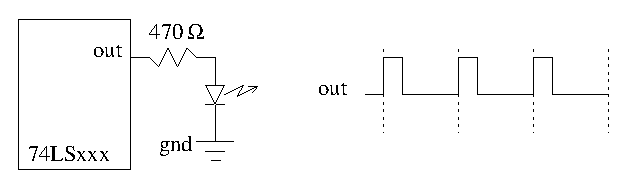
\includegraphics{pulse}}
                        \caption{An active high LED and the waveform driving it.}
                        \label{fig:commonPeripheralComponentspulse}
                    \end{figure}

                    The only point that remains is to discuss the fundamental frequency of
                    the waveform being applied to the LED.  Clearly, a frequency of 1hz
                    will be perceived as a visible blinking on and off.  If however the
                    frequency is pushed above 60hZ, the fastest frequency detectable by humans,
                    then something apparently miraculous happens.  The rapid blinking disappears
                    and is replaced with a steady glow.  As the average power dissipated by the
                    LED increases so does the perceived illumination level.

                    \section{Alphanumeric Display}
                    \index{alphanumeric display|(}
                        \label{page:alpha}
                        \begin{buildingblock}{Alphanumeric Display }
                            \begin{tabular}{|l|p{3.5in}|} \hline
                                Nomenclature:  & 14-segment Alphanumeric Display  \\ \hline
                                Data Input:    & 14-bits A,B,...,N     \\ \hline
                                Data Output    & none    \\ \hline
                                Control:       & none           \\ \hline
                                Status:        & none                                   \\ \hline
                                Physical Input:& none        \\ \hline
                                Physical Output:& light pattern        \\ \hline
                                Others:        & none                   \\ \hline
                                Behavior:      & when data input is high corresponding segment
                                is illuminated. \\ \hline
                            \end{tabular}
                        \end{buildingblock}

                        The 14-segment alphanumeric display is just a variation on the
                        7-segment display discussed on page \pageref{page:7seg}.  The addition
                        of 7 extra illuminating segments to the 7-segment display gives
                        it the capability of displaying a range of letters as well as
                        numbers.  Figure~\ref{fig:commonPeripheralComponentsalpha}A shows the arrangement of segments
                        and their designations.  In Figure~\ref{fig:commonPeripheralComponentsalpha}B three displays
                        are used together to form the word "BIT".

                        \begin{figure}[ht]
                            \center{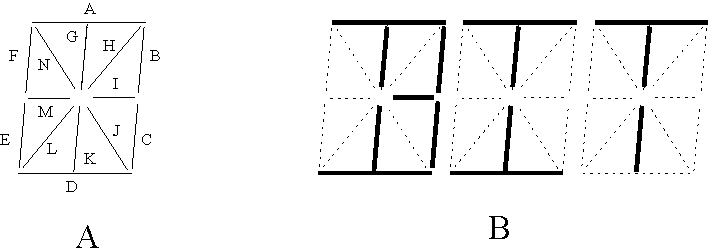
\includegraphics{alpha}}
                        \caption{A) The arrangement of segments and their designations.  B) Three
                    displays forming the word "BIT".}
                    \label{fig:commonPeripheralComponentsalpha}
                \end{figure}

                Its important to note that both the 7 and 14 segment displays are
                merely a collection of LEDs placed in the same package.  Its impractical
                and unnecessary to route both ends of every LED out to the package.
                Typically either the anode or cathode of every LED in a display is
                tied together
                and routed outside the package.  If all the cathodes are collected
                together then the displays is called a common cathode display.  If
                all the anodes are collected together then the displays is referred
                to as a common anode.  Figure~\ref{fig:commonPeripheralComponentscommon} shows a common
                cathode display.
                \index{common anode|(}
                    \index{common cathode|(}

                        \begin{figure}[ht]
                            \center{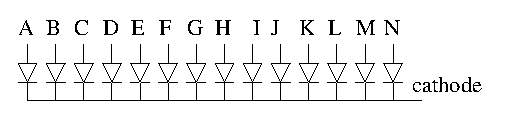
\includegraphics{common}}
                            \caption{A schematic of a 14-segment common cathode display.}
                            \label{fig:commonPeripheralComponentscommon}
                        \end{figure}

                        \section{Hall Effect Sensor}
                        TBD

                        \section{Infrared Range Finder}
                        TBD

                        \section{Ultrasonic Range Finder}
                        \index{Ultrasonic sensor|(}
                            \label{page:ultrasonic}
                            \begin{buildingblock}{Ultrasonic Range Finder}
                                \begin{tabular}{|l|p{3.5in}|} \hline
                                    Nomenclature:  & ultrasonic sensor  \\ \hline
                                    Data Input:    & 1-bit Enable     \\ \hline
                                    Data Output:   & 1-bit Echo   \\ \hline
                                    Control:       & none           \\ \hline
                                    Status:        & none                                   \\ \hline
                                    Physical Input:& echo of audio output        \\ \hline
                                    Physical Output:& high frequency audio chirp        \\ \hline
                                    Others:        & none                   \\ \hline
                                    Behavior:      & When enable make a positive edge transition
                                    a ultrasonic chirp is generated by the transducer.  When the
                                    transducer detects an echo it sends the corresponding output hi. \\ \hline
                                \end{tabular}
                            \end{buildingblock}

                            Ultrasonic range finders are useful when you need a device which
                            can detect the absence or presence of an object over a 20 foot
                            range regardless of the lighting conditions.   As their name implies,
                            an ultrasonic range finder does this by sending out a sound wave
                            and then listening for the return echo.  This sound can be heard (and
                            felt) by humans and will be refereed to as a chirp.
                            Figure~\ref{fig:commonPeripheralComponentsultra} shows the transducer generating a chirp in
                            response to enable going high, the resulting sound striking the
                            hexagon and then returning back to the transducer.  This return
                            sound would cause the echo signal to go to logic 1.

                            \begin{figure}[ht]
                                \center{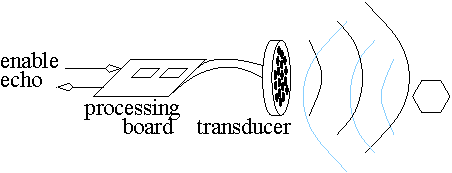
\includegraphics{ultra}}
                                \caption{An ultrasonic range finder.}
                                \label{fig:commonPeripheralComponentsultra}
                            \end{figure}

                            Given that the transducer is performing both transmit and receive
                            roles, hence the name transducer, it has to be careful not to get
                            the two confused.  This can
                            happen if the processing board tries to "listen" to the transducer
                            immediately after the transducer has generated a chirp.  In this case
                            the processing board may interpret the residual transducer vibration
                            caused in the process of generating a chirp as an echo.  Consequently,
                            ultrasonic range finders
                            usually have a minimum range, objects closer than this cannot be detected.

                            You may be asking yourself, "how can detecting an echo help me determine
                            the distance to an object?"  Since sound travels at a know speed
                            then knowing how long it took the sound to travel
                            to an object and back can be used to determine the distance.  If we assume
                            that it takes X seconds to travel to an object and back then the distance
                            to the object is given by the equation below.

                            $$    \frac{779 \text{ \ miles}}{\text{ \ hour}} *
                            \frac{1 \text{ \ hour}} {3600 \text{ \ seconds}} *
                            \frac{5280 \text{ \ feet}}{\text{ \ mile}} *
                            \frac{X \text{ \ seconds}}{2} =
                            X * 571 \text{ \ feet} $$

                            The factor of X/2 results from the fact that X is the time to the
                            object and back, whereas X/2 is the time required to reach the object.

                            %% motion output devices

                            \section{DC Motor}
                            \index{motor!dc}
                            \label{page:dvmotor}
                            \begin{buildingblock}{DC motor}
                                \begin{tabular}{|l|p{3.5in}|} \hline
                                    Nomenclature:  & DC motor  \\ \hline
                                    Data input:    & none    \\ \hline
                                    Data output:   & none     \\ \hline
                                    Control:       & none     \\ \hline
                                    Status:        & none      \\ \hline
                                    Physical Input:& none        \\ \hline
                                    Physical Output:& rotating shaft        \\ \hline
                                    Others:        & 2 leads $V_l, V_r$      \\ \hline
                                    Behavior:      & When $V_l-V_r > 0$ the output shaft rotates clockwise,
                                    when $V_l-V_r < 0$ the output shaft rotates counterclockwise, otherwise the
                                    output shaft does not rotate. \\ \hline
                                \end{tabular}
                            \end{buildingblock}

                            Because of the way that a DC motor is built, its speed is determined
                            by the potential difference between its leads.  Reversing the
                            potential between the leads will cause the axle to rotate
                            in the opposite direction.  Its also
                            important to note that turning the axle of a DC motor will
                            cause a potential to develop between the two leads.

                            The voltages and currents required to run most DC motors is
                            far beyond the capabilities of a digital circuit.  A specific
                            type of amplifier called an H-bridge can be used as an interface
                            between digital electronics and a DC motor.  An H-bridge can be
                            constructed from MOSFETs as shown in
                            Figure~\ref{fig:commonPeripheralComponentshbridge}.  An H-bridge derives its name from
                            this  H-shaped schematic.  The main function of an H-bridge is
                            to allow the potential across the motor to be either positive,
                            negative, or zero.  Lets assume that the MOSFETs shown in
                            Figure~\ref{fig:commonPeripheralComponentshbridge} have a low resistance between source and
                            drain when the gate is at logic 1 and have a high resistance
                            otherwise.  If $L_1,L_0 = 1,0$ and $R_1,R_0 = 0,1$ then the
                            potential difference is $V_l - V_r > 0$.
                            Figure~\ref{fig:commonPeripheralComponentshbridge}B shows the resulting flow of current.
                            If $L_1,L_0 = 0,1$ and $R_1,R_0 = 1,0$ then the
                            potential difference $V_l - V_r < 0$.  The resulting flow of
                            current is shown in Figure~\ref{fig:commonPeripheralComponentshbridge}C.
                            If $L_1,L_0 = 0,0$ and $R_1,R_0 = 0,0$ then the potential difference
                            $V_l - V_r < 0$. When none of the H-bridge arms is active we say that
                            the motor is coasting because the output shaft
                            can be turned by an external force.  An H-bridge is designed
                            to run a DC motor at full speed forward or backwards.  In order
                            to run a DC motor at variable speed the control signals should be PWM
                            between the required direction and coast.

                            \begin{figure}[ht]
                                \center{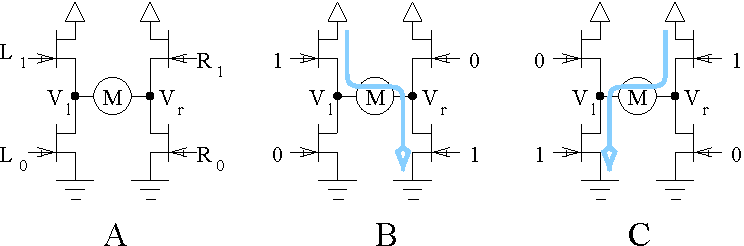
\includegraphics{hbridge}}
                                \caption{An H-bridge driving a DC motor.}
                                \label{fig:commonPeripheralComponentshbridge}
                                \index{motor!H-bridge}
                            \end{figure}

                            There are at least two problems with the schematic in
                            Figure~\ref{fig:commonPeripheralComponentshbridge} which would prevent it form working.
                            First, 0 and 5 volts may be insufficient to turn on the MOSFETs.
                            This problem can be resolved by amplifying the digital signal
                            using a single-rail op-amp (LM364) in an open loop configuration.
                            The second problem arises whenever the H-bridge transitions
                            from driving the motors to coasting.  Under such a condition, the
                            output shaft of the DC motor will continue to spin due to the
                            inertial properties of the load.  As noted earlier turning the
                            axle of a DC motor creates a potential difference between the
                            motors leads.  If this potential difference becomes too
                            large it will destroy the MOSFETs.
                            This problem can be averted by placing (flyback) diodes from the
                            source to drain of each of the four MOSFETs to shunt this excess
                            current directly to the power supply.

                            \section{Stepper motor}
                            \index{motor!stepper}
                            \label{page:stepper}
                            \begin{buildingblock}{Stepper Motor}
                                \begin{tabular}{|l|p{3.5in}|} \hline
                                    Nomenclature:  & stepper motor \\ \hline
                                    Data Input:    & none     \\ \hline
                                    Data Output    & none    \\ \hline
                                    Control:       & 4 stator controls a,b,c,d  \\ \hline
                                    Status:        & none                                   \\ \hline
                                    Physical Input:& none        \\ \hline
                                    Physical Output:& rotating shaft \\ \hline
                                    Others:        & none                   \\ \hline
                                    Behavior:      & when controls are sequenced correctly the
                                    motor turns CW or CCW. \\ \hline
                                \end{tabular}
                            \end{buildingblock}

                            All electric motors operate on two basic principles;
                            current flowing through a loop of wire creates a magnetic
                            field and opposite magnetic fields attract.
                            The output shaft of a stepper motor is connected to a permanent
                            magnetic.  The four control wires are connected to stators which
                            are arranged around this magnet.  By applying a voltage to a
                            control wire, magnetic field is created in the stator
                            attracting the opposite pole of the permanent magnet, turning
                            the motors axle.  The trick with a stepper motor is generating
                            the correct sequence to turn the motor.  Knowing what's inside
                            the stepper motor will help in developing the drive sequence.
                            Figure~\ref{fig:commonPeripheralComponentsstepper} shows the internal organization of a
                            stepper moor.

                            \begin{figure}[ht]
                                \center{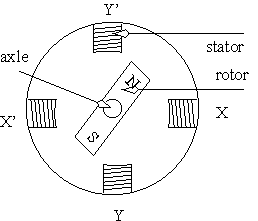
\includegraphics{stepper}}
                                \caption{The internal organization of a stepper motor.}
                                \label{fig:commonPeripheralComponentsstepper}
                            \end{figure}

                            The permanent magnet on the rotor seeks the induced magnetic field
                            created on the stator.  Magnetic fields are created on the stator
                            when the user applies a positive or negative voltage.  Lets assume
                            that a logic 1 on the stator input creates a south magnetic field facing the rotor
                            and north field facing outwards from the motor.  A logic 0 on an input
                            will create a north magnetic field towards the rotor and a south magnetic
                            field orient away from the motor.  In Figure ~\ref{fig:commonPeripheralComponentsstepper}
                            the input $x,x',y,y' = 0,1,0,1$ causes the associated stators to generate
                            $N,S,N,S$ magnetic fields towards the rotor.  Since opposite magnetic
                            fields attract then the rotor in the figure will feel a counterclockwise
                            rotational force.  Once the south end of the rotor's magnet reaches the
                            north stator the motor will stop moving.  In order to keep moving
                            the rotor a new input must be applied.  Table~\ref{table:stepper}
                            describes the inputs and the resulting angle of the rotor.

                            \begin{table}
                                \begin{tabular}{l|l|l|l||l}
                                    x    & x'    & y    & y'    & rotor angle \\ \hline
                                    0    & 1    & 0    & 1    & 0 degrees \\ \hline
                                    1    & 0    & 0    & 1    & 90 degrees \\ \hline
                                    1    & 0    & 1    & 0    & 180 degrees \\ \hline
                                    0    & 1    & 1    & 0    & 270 degrees \\
                                \end{tabular}
                                \label{table:stepper}
                                \caption{A typical step sequence for a stepper motor. Not so
                                ordinary stator angles for each step value.}
                            \end{table}

                            In reality each input is attached to a collection of stators inside the motor.
                            Thus, the stators are arranged in sequence
                            $x',y',x,y,x',y',...$ around the perimeter of the motor.  Hence,
                            each step of the motor will produce a small deflection of the
                            rotor as opposed to the 90 degree deflection shown in
                            Table~\ref{table:stepper}.  Stepper motors are used in applications
                            that require very precise mechanical rotation; each step sequence
                            produces a known and repeatable deviation in the axle's angle.
                            Stepper motors do not produce much torque and are typically a poor
                            choice for the main drive motors in robots.

                            \section{Servo motor}
                            \index{motor!servo}
                            \label{page:servo}
                            \begin{buildingblock}{Servo Motor}
                                \begin{tabular}{|l|p{3.5in}|} \hline
                                    Nomenclature:  & servo motor  \\ \hline
                                    Data input:    & none    \\ \hline
                                    Data output:   & none     \\ \hline
                                    Control:       & 1-bit control     \\ \hline
                                    Status:        & none      \\ \hline
                                    Physical Input:& none        \\ \hline
                                    Physical Output:& position shaft    \\ \hline
                                    Others:        & \VCC and GND     \\ \hline
                                    Behavior:      & The angular position of the axle is set by the time
                                    high of the control signal. \\ \hline
                                \end{tabular}
                            \end{buildingblock}

                            Servo motors can only move their output shafts through 180 degrees.
                            They are not manufactured to turn continuously like a DC or stepper motor
                            (though they can be modified to do so).  Generally, servo motors are used
                            to move a load to a specific position.  The pulse width of the control signal
                            determines the position of the axle as shown in the following table.

                            \begin{tabular}{l|l}
                                Pulse width & angle    \\    \hline \hline
                                1.0ms        & 0 degrees    \\    \hline
                                1.75ms        & 90 degrees    \\    \hline
                                2.5ms        & 180 degrees    \\
                            \end{tabular}

                            Each pulse of the control signal is said to \textit{ refresh} the servo's
                            output.  Typically, the output of a servo motor is refreshed at around
                            20Hz.  Between consecutive refreshes the servo motors' output shaft
                            may be deflected by the load. Thus, the refresh rate must be sufficient
                            to cancel these deflections.

                            Servo motors are simple to use because the servo motor contains all the
                            control and power circuitry.  All the user has to do is provide power
                            and send in  a control signal to control the motors position.

                            \section{Liquid Crystal Display}
                            \index{LCD}
                            \label{page:lcd}

                            \begin{buildingblock}{Liquid Crystal Display}
                                \begin{tabular}{|l|p{3.5in}|} \hline
                                    Nomenclature:  & Liquid Crystal Display  \\ \hline
                                    Data input:    & 8-data bits  \\ \hline
                                    Data output:   & none     \\ \hline
                                    Control:       & 3-bits E, RS, R/W'     \\ \hline
                                    Status:        & none      \\ \hline
                                    Physical Input:& none        \\ \hline
                                    Physical Output:& none    \\ \hline
                                    Others:        & \VCC and Gnd     \\ \hline
                                    Behavior:      & Displays the ASCII character sent or
                                    performs some display configuration. \\ \hline
                                \end{tabular}
                            \end{buildingblock}

                            What you take for a LCD really consists of two parts; a LCD and a controller
                            chip.   The LCD is the glass that you see
                            characters on. The LCD contains something like 80 wires that are used
                            to draw all pixels on the display. The
                            controller chip reduces all this control information down to 14-pins.
                            Most LCD's have a Hitachi compatible controller chip. The technical
                            documentation for this driver can be found online.

                            The controller makes the LCD act like a 80 bytes RAM where each location
                            in the RAM corresponds to one of the character positions in the 40 column
                            by 2 row display space.  The ASCII value of the byte stores at location X
                            is the character displayed in the LCDs display space.  For example, storing
                            0x5A (The character "Z") at location 0 will result in a "Z" beign displayed
                            in the upper left corner of the display.  Since the LCD's physical display
                            is 16x2 then only a portion of the display space can be seen at a time. The
                            viewable region will be called the "window" on the LCD's memory.

                            Characters are written to the LCD by manipulating the 3 control signals and
                            the data lines.  The R/W' signal is a read write signal.  Since there are
                            a single set of data lines then care must be taken to prevent short circuits
                            when reading and writing to the LCD.  The register select or RS signal
                            determines the meaning of the data.  RS=0 allows access to the control and
                            status registers of the LCD.  RS=1 gives the user access to the data RAM
                            of the LCD.  The E signal must be strobed high in order to complete a
                            data transaction to/from the LCD.  An LCD typically requires about 40uS
                            to complete a typical operation before being able to receive the next
                            command.

                            \section{Remote Control Decoder}
                            \index{Remote control}
                            \label{page:remote}
                            \begin{buildingblock}{Remote Control Decoder}
                                \begin{tabular}{|l|p{3.5in}|} \hline
                                    Nomenclature:  & Remote control decoder  \\ \hline
                                    Data input:    & none  \\ \hline
                                    Data output:   & 1-bit data     \\ \hline
                                    Control:       & none     \\ \hline
                                    Status:        & none      \\ \hline
                                    Physical Input:& none        \\ \hline
                                    Physical Output:& none    \\ \hline
                                    Others:        & \VCC and GND     \\ \hline
                                    Behavior:      & Decodes a serial data packet sent by
                                    a remote control. \\ \hline
                                \end{tabular}
                            \end{buildingblock}

                            Remote control signals are sent by encoding bursts of infrared light.  A logic
                            0 is sent by pulsing infrared (940nm to be precise) light on and off at 38KHz;
                            via an infrared LED, commonly called an IRED.
                            A logic 1 is sent by transmitting no infrared light at all.  The 38KHz signal
                            is called the carrier frequency of the signal, this means that this high frequency
                            signal carries the information, rather than being the information itself.  The
                            remote control decoder is a small device with 3-pins; \VCC, GND, and data.  The
                            data line is the demodulated to produce a sequence of 0's and 1's.  Well, what do
                            these bits mean?

                            The answer depends on what kind of remote control is sending the signal.  In the
                            case of a RCA remote, a single bit is represented by holding the data line low and
                            then holding the data line high.  The time low is always 1ms.  The time high is
                            either 0.5ms for a logic 0 , or 1.5mS for a logic 1.  An RCA packet starts with
                            a start bit which has an especially long period of 5ms.  Following the start
                            bit are 24 data bits representing a single 12-bit data packet.  The 12-bits
                            which encode the key pressed are sent and then their complement is sent, this
                            enables a simple form of error checking to be performed, check that the every
                            bit in one subpacket has a negation in the subsequent subpacket.  After the 24-data
                            bits comes a single stop bit.

                            You might wonder, why an engineer would modulate a logic 0 at 38KHz, rather than
                            just send turn the IR beam on for a 1 and turn it off for a 0.  There are three
                            good reasons to modulate the signal.  The first is that
                            it reduces the chances of the receiver confusing ambient light from the
                            signal in questions; few phenomena in nature emit 940nM radiation at 38KHz. The
                            second is that it saves energy; when transmitting a 0, the IR beam only need be
                            on for a very short period of time.  The third reason is that it actually
                            increases the range of the IR beam.  Typically, the IR beam has a 5\% duty cycle,
                            meaning the IRED is only on 5\% of the time.  However, during it on time,
                            as much current as possible is pumped through the IRED.  The remaining 95\% of
                            the time is given over to allowing the IRED to cool down.  Thus you get a really
                            bright pulse of radiation which can be detected far away.

                            \section{CRT}
                            \index{crt}
                            \label{page:crt}
                            \begin{buildingblock}{Cathode Ray Tube}
                                \begin{tabular}{|l|p{3.5in}|} \hline
                                    Nomenclature:  & Cathode Ray Tube  \\ \hline
                                    Data input:    & Red, Green, Blue (RGB)   \\ \hline
                                    Data output:   & none     \\ \hline
                                    Control:       & vsynch, hsynch     \\ \hline
                                    Status:        & none      \\ \hline
                                    Physical Input:& none        \\ \hline
                                    Physical Output:& Character display    \\ \hline
                                    Others:        & 120 VAC     \\ \hline
                                    Behavior:      & The RGB colors are painted across the display 1 row
                                    at a time according to vsynch and hsynch. \\ \hline
                                \end{tabular}
                            \end{buildingblock}

                            Since 1980 the Video Graphics Array or VGA standard has been the
                            standard interface to computer displays. This standard has enjoyed
                            popular success because it provides high resolution, rich color,
                            in an easy to use interface. The VGA standard breaks the screen
                            into 640 columns by 480 rows. Each point on the screen is called a
                            picture element or pixel for short. The interface to a VGA display
                            is based on the technology used to draw images on the display. A
                            B\&W display contains an electron gun which fires negatively charged
                            particles at a phosphorous coating inside a Cathode Ray Tube (CRT).
                            When electrons strike the phosphorous coating they create a momentary
                            glow. By rapidly steering the electron gun across the display, while
                            simultaneously turning the electron gun on and off, creates a single
                            line of an image. After the end of the line is reached the electron
                            gun is sent back across the display. A complete image is formed by
                            rapidly drawing lines one after another down the CRT. After drawing
                            a frame of data, the electron gun must be sent back to the top of the
                            display.

                            A color display operates just like a B\&W display except that it contains
                            three electron guns. Each gun is aimed a a particular sub-region of a
                            pixel; the phosphorous in each subpixel responds by generating either
                            red, green or blue light.

                            So how exactly do the r,g,b signals combine to form colors? Well
                            video colors mix in exactly the opposite way that paints mix. When
                            you mix together a lot of different color paints you generally end
                            up with a very dark color approaching black. However, when you mix
                            together a lot of video colors you generally end up with a light
                            color approaching white. The table below shows the 8 combinations
                            of r,g,b when they are represented by a single bit.

                            \begin{table}[ht]
                                \center{
                                    \begin{tabular}{cc}
                                        RGB & color \\ hline
                                        000 & black \\ \hline
                                        001 & blue  \\ \hline
                                        010 & green \\ \hline
                                        011 & turquoise \\ \hline
                                        100 & red \\ \hline
                                        101 & magenta \\ \hline
                                        110 & yellow \\ \hline
                                        111 & white \\
                                \end{tabular} }
                            \end{table}

                            It remains to explain how the timing of vsynch and hsynch signals
                            line up to the pixels displayed on the screen.  Lets imagine that
                            the display has just finished drawing a individual line of pixels
                            and that the pixel gun is pointed off the right side of the display.
                            The main role of the hsynch signal is to tell the CRT to point the
                            pixel gun back to the left side of the screen.  You do this by pulsing
                            the hsynch signal low for 3.77us.  You then need to wait 1.89uS for
                            the pixel gun to actually reach the left side of the screen, this is
                            termed the "Back porch".  You then have 25.17uS to output all 640 pixels
                            that form that scan row.  Since each pixel should be displayed in
                            the same amount of time, each should take 0.0394uS.  After the scanline
                            pixels have been displayed you should wait 0.94 uS before dropping
                            the hsynch signal low.  It would behoove the digital designer to make
                            the main clock frequency of any device which controls the pixel gun to
                            be a multiple of the pixel duration.

                            The vsynch signal works in much the same way that the hsynch signal
                            does, except that it deals with longer periods of time.  As the CRT
                            draws successive scanlines it works its way down the CRT.  Lets assume
                            that the CRT has just completed drawing an entire screens worth of
                            data and that we want to start again.  In order to move the pixel gun
                            back to the top of the display, the vsynch signal should be held low
                            for 15.58ms.  After this you need to wait 1.02mS before starting to
                            draw the first scanline.  The CRT then draws 480 successive scanlines
                            all the while vsynch should be held at logic 1.  After drawing all 480
                            scanline, you should wait 0.35mS before strobing vsynch low, ending the
                            current frame of video.

                            %% Circuits
                            %% communication
                            %% \section{InfraRed transmitter/receiver}
                            %% \section{IrDA}
                            %\section{Analog to Digital Converter}
                            %\section{Digital to Analog Converter}
                            % Arb Logic circuits
                            %\section{Field Programmable Gate Arrays}
                            %% \section{GALs}
                            %% \section{PLAs}
                            %\section{Protocols}
                            %\subsection{RS232}
                            %\subsection{I2C}
                            %\subsection{Universal Serial Bus}
                            %% Physical environment
                            %% \section{Thermometer}
                            %% \section{Photoresistor}
